\documentclass[12pt, a4paper]{article}

\usepackage{amsmath}
\usepackage{array}
\usepackage[portuguese]{babel}
\usepackage{chngpage}
\usepackage{float}
\usepackage[a4paper, margin=2cm]{geometry}
\usepackage{graphicx}
\usepackage{hyperref}
\usepackage{setspace}
\usepackage{xcolor}

\title{\Huge \textbf{Computação Gráfica \\ \Large Trabalho Prático -- Fase I}}
\date{2 de março 2025}
\author{Grupo 3}

\begin{document}

\begin{center}
    
\includegraphics[width=0.25\textwidth]{res/cover/EE-C.eps}
\end{center}

\chardef\_=`_
\onehalfspacing
\setlength{\parskip}{\baselineskip}
\setlength{\parindent}{0pt}
\def\arraystretch{1.5}

{\let\newpage\relax\maketitle}
\maketitle
\thispagestyle{empty}

\vspace*{\fill}

\begin{adjustwidth}{-2cm}{-2cm} % These values only need to be large enough to center the table
    \begin{center}
        \begin{tabular}{>{\centering}p{0.25\textwidth}
                        >{\centering}p{0.25\textwidth}
                        >{\centering}p{0.25\textwidth}
                        >{\centering\arraybackslash}p{0.25\textwidth}}
            
\includegraphics[width=3.5cm]{res/cover/A104437.png} &
            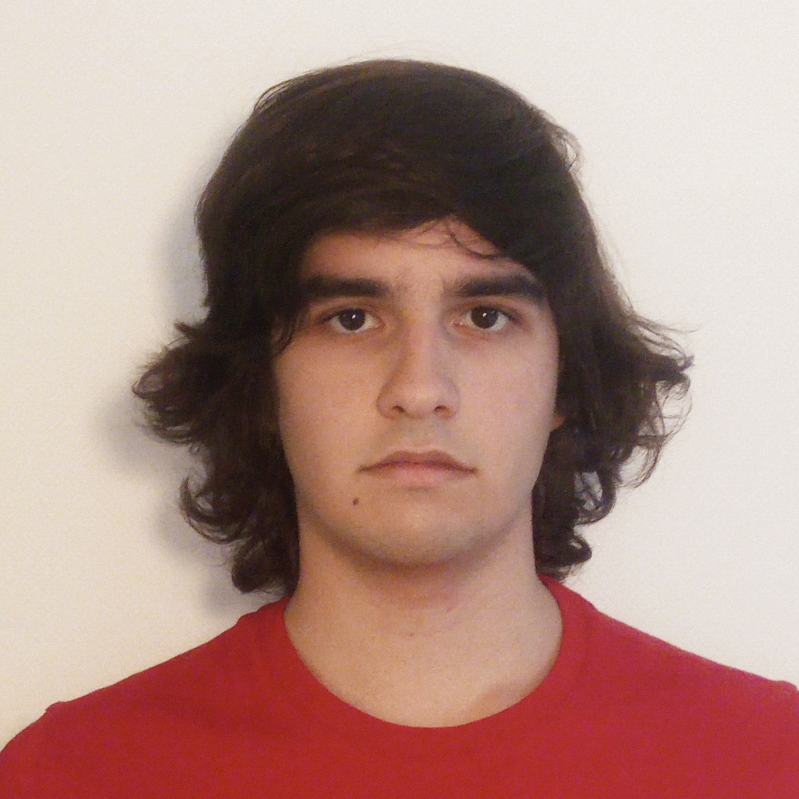
\includegraphics[width=3.5cm]{res/cover/A104348.png} &
            
\includegraphics[width=3.5cm]{res/cover/A90817.png} &
            
\includegraphics[width=3.5cm]{res/cover/A104179.png} \\

            Ana Oliveira & Humberto Gomes & Mariana Cristino & Sara Lopes \\
            A104437      & A104348        & A90817           & A104179
        \end{tabular}
    \end{center}
\end{adjustwidth}

\pagebreak

\begin{abstract}
    \textbf{\color{red} TODO - resumo}
\end{abstract}

\section{\emph{Generator}}

\subsection{Descrição e uso}

\textbf{\color{red} TODO - descrição e uso do programa}

\subsection{Formato \texttt{.3d}}

Visto que a estrutura de um ficheiro \texttt{.3d} separa os vértices de um modelo das suas faces, o
processo de criação dos modelos 3D dos vários sólidos é dividido em duas fases: a geração do
conjunto de pontos que os constituem, e o seu agrupamento em faces triangulares.

\subsection{Plano}

O primeiro passo para a geração da nuvem de pontos de um plano é o cálculo do comprimento de uma
divisão, $d = \frac{L}{N}$, onde $L$ simboliza o comprimento do plano e $N$ o número de divisões.
Depois, determinam-se os dois vetores que definem a direção do plano. Estes poderiam ser os vetores
diretores dos eixos $x$ e $z$, mas é mais simples que estes tenham o comprimento de uma divisão do
plano.

$$
\vec{\imath} = (d, 0, 0)
\hspace{1cm}
\vec{\jmath} = (0, 0, d)
$$

Depois, encontra-se o ponto do plano com os menores valores das coordenadas $x$ e $z$. Como se
deseja que o plano esteja centrado na origem, as coordenadas $x$ e $z$ do ponto desejado serão o
simétrico da metade do comprimento do plano:

$$
P_0 = \left ( - \frac{L}{2}, 0, - \frac{L}{2} \right )
$$

Depois, qualquer ponto $P$ do plano pode ser definido como a adição a $P_0$ de uma combinação linear
de $\vec{\imath}$ e $\vec{\jmath}$, limitando a números inteiros os coeficientes multiplicativos dos
vetores:

$$
P = P_0 + \alpha \, \vec{\imath} + \beta \, \vec{\jmath}
\hspace{1cm}
\alpha, \beta \in \left \lbrace 0, 1, \ldots, N \right \rbrace
$$

Na prática, o plano é gerado iterando pelos valores inteiros possíveis de $\alpha$ e de $\beta$,
incrementando primeiro $\beta$, e só depois de $\alpha$, o que dá origem a uma nuvem de pontos como
a que pode ser observada na figura abaixo:

\begin{figure}[H]
    \centering
    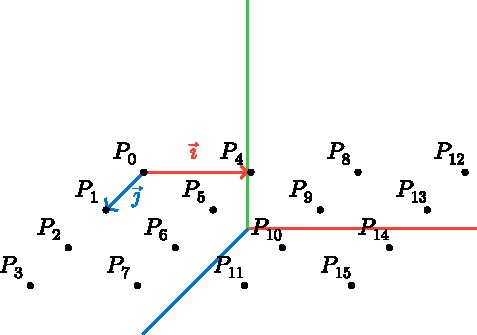
\includegraphics[width=0.4\textwidth]{res/figures/PlanePoints.pdf}
    \caption{Nuvem de pontos resultante da geração de um plano de três divisões.}
\end{figure}

Depois, os vértices gerados podem ser agrupados nos triângulos que formam o plano. Para tal,
começa-se com o primeiro vértice do plano, $P_0$. Considera-se também o vértice seguinte, $P_1$, e
os dois vértices com os valores de $z$ de $P_0$ e $P_1$, mas com o seguinte valor de $x$ possível
(na "linha"{} seguinte). Um exemplo de um conjunto destes quatro vértices pode ser visto na figura
abaixo. Com estes vértices, gera-se um quadrado, ou seja, dois triângulos. Este processo repete-se
para todos os vértices onde é aplicável, ou seja, todos com exceção dos pontos com os maiores
valores de $x$ ou de $z$ possíveis.

\begin{figure}[H]
    \centering
    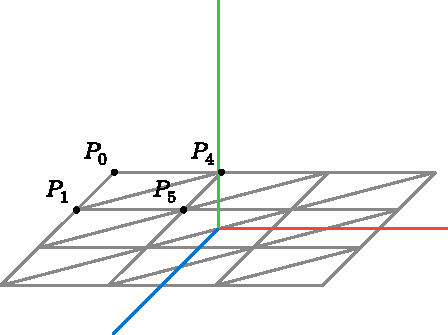
\includegraphics[width=0.4\textwidth]{res/figures/PlaneTriangles.pdf}
    \caption{
        Triângulos de um plano gerado, e pontos utilizados na primeira iteração do ciclo de geração
        de triângulos.
    }
\end{figure}

Uma otimização feita pela \emph{engine} é \emph{face culling}, ou seja, desenhar apenas as faces
voltadas para a câmara. No caso do plano, deseja-se que os seus triângulos estejam voltados para
cima, pelo que os seus vértices devem estar ordenados na ordem contrária à dos ponteiros do
relógio. Para os quatro pontos apresentados acima, os triângulos gerados são os seguintes:

$$
T_1 = (P_1, P_4, P_0)
\hspace{1cm}
T_2 = (P_1, P_5, P_4)
$$

\subsection{Cubo}

De um modo simples, o processo de geração de um cubo consiste na repetição da geração de um plano
seis vezes, uma vez para cada face. No entanto, algumas diferenças devem ser evidenciadas. Tal como
no plano, após ser calculado o comprimento de uma divisão do cubo, são definidos os vetores
diretores dos vários planos que são as faces do cubo. Há três pares de vetores diretores, cada um
utilizado para gerar duas faces opostas:

$$
\begin{array}{ll>{\hspace{1cm}}ll>{\hspace{1cm}}c}
    \vec{\imath_1} &= (1, 0, 0) &
    \vec{\jmath_1} &= (0, 1, 0) &
    (\text{faces dianteira e traseira}) \\
    \vec{\imath_2} &= (0, 1, 0) &
    \vec{\jmath_2} &= (0, 0, 1) &
    (\text{faces esquerda e direita}) \\
    \vec{\imath_3} &= (0, 0, 1) &
    \vec{\jmath_3} &= (1, 0, 0) &
    (\text{faces superior e inferior})
\end{array}
$$

Ao contrário do que acontece no plano, estes vetores encontram-se normalizados, o que é útil para
determinar o ponto de cada face a partir do qual os seus restantes pontos serão gerados. Tal como
acontece no plano, para o cubo estar centrado na origem, é necessário que todas as coordenadas deste
ponto inicial estejam a uma distância de $\frac{L}{2}$ da origem, onde $L$ representa o comprimento
do lado do cubo. Por exemplo, para o primeiro par de vetores diretores, os pontos são os seguintes,
correspondentes às faces traseira e dianteira, respetivamente:

$$
P_{0^-} = \left ( -\frac{L}{2}, -\frac{L}{2}, -\frac{L}{2} \right )
\hspace{1cm}
P_{0^+} = \left ( -\frac{L}{2}, -\frac{L}{2}, +\frac{L}{2} \right )
$$

De um modo geral, nas coordenadas onde $\vec{\imath}$ ou $\vec{\jmath}$ têm um valor não nulo, a
coordenada do ponto inicial é $-\frac{L}{2}$. A coordenada restante pode assumir, conforme a face,
ou $\frac{L}{2}$ ou $-\frac{L}{2}$. Matematicamente, o vetor perpendicular à face é dado por:

$$
\vec{n} = (1, 1, 1) - \vec{\imath} - \vec{\jmath}
$$

A partir deste vetor, os pontos iniciais das faces são dados por:

$$
P_{0^-} = -\frac{L}{2} \left ( \vec{\imath} + \vec{\jmath} + \vec{n} \right )
\hspace{1cm}
P_{0^+} = -\frac{L}{2} \left ( \vec{\imath} + \vec{\jmath} - \vec{n} \right )
$$

Com os vetores diretores e os pontos iniciais de cada face, é possível normalizar os vetores
diretores e gerar os pontos de cada face, seguindo o mesmo processo utilizado para o plano. Abaixo,
apresenta-se um exemplo da nuvem de pontos de um cubo gerado:

\begin{figure}[H]
    \centering
    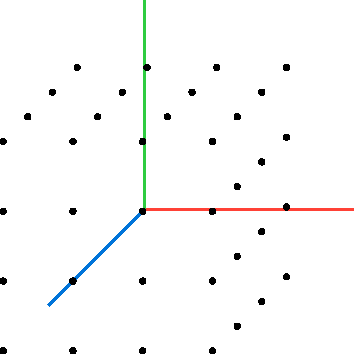
\includegraphics[width=0.35\textwidth]{res/figures/CubePoints.pdf}
    \caption{
        \onehalfspacing
        Nuvem de pontos resultante da geração de um cubo de três divisões. Os pontos das faces
        ocultas não foram representados nesta figura.
    }
\end{figure}

Depois de gerada a nuvem de pontos, o processo de geração dos triângulos de cada face é muito
semelhante ao do plano. No entanto, a ordem dos vértices de cada triângulo difere conforme a face do
cubo a ser construída. Considere-se o exemplo abaixo, o das faces superior e inferior de um cubo com
apenas uma divisão:

\begin{figure}[H]
    \centering
    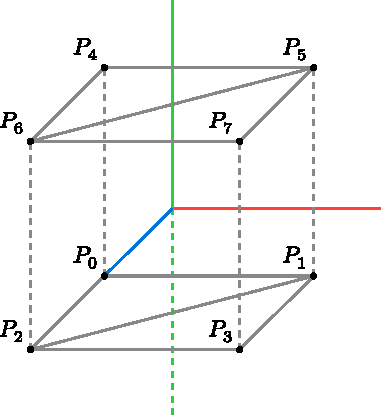
\includegraphics[width=0.35\textwidth]{res/figures/CubeFaces.pdf}
    \caption{Faces superior e inferior de um cubo de apenas uma divisão.}
\end{figure}

Para que os triângulos da face inferior estejam voltados para o exterior do cubo, ou seja, para
baixo, os seus pontos são ordenados no sentido dos ponteiros do relógio:

$$
T_1 = (P_1, P_2, P_0)
\hspace{1cm}
T_2 = (P_1, P_3, P_2)
$$

Na face superior, a ordem dos pontos dos triângulos é contrária, no sentido contrário ao dos
ponteiros do relógio:

$$
T_1' = (P_5, P_4, P_6)
\hspace{1cm}
T_2' = (P_7, P_5, P_6)
$$

Para cada par de faces opostas, cada face será sujeita, conforme o seu vetor normal, a uma ordenação
distinta dos pontos dos seus triângulos. Após aplicar o processo de geração de triângulos a todas as
faces, é dada por concluída a construção do modelo do cubo.

\begin{figure}[H]
    \centering
    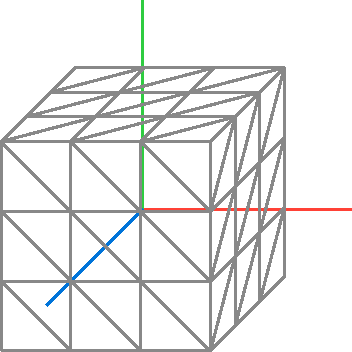
\includegraphics[width=0.35\textwidth]{res/figures/CubeTriangles.pdf}
    \caption{
        \onehalfspacing
        Triângulos resultantes da geração de um cubo de três divisões. As faces ocultas não foram
        representadas nesta figura.
    }
\end{figure}

\section{\emph{Engine}}

\textbf{\color{red} TODO - \emph{engine}}

\section{Resultados obtidos}

\textbf{\color{red} TODO - resultados}

\section{Conclusão e Trabalho Futuro}

\textbf{\color{red} TODO - conclusão}

\begingroup
\section{Bibliografia}
\renewcommand{\section}[2]{}

\begin{thebibliography}{9}
    \bibitem{exemplo}
        \href{https://youtu.be/dQw4w9WgXcQ}{Um item de exemplo na bibliografia}
\end{thebibliography}
\endgroup

\end{document}
